\documentclass[10pt,conference]{IEEEtran}
\IEEEoverridecommandlockouts

\usepackage{graphicx}
\usepackage{amsmath}
\usepackage{xcolor}
\usepackage{booktabs}
\usepackage{tabularx}
\usepackage{array}
\usepackage{capt-of}
\usepackage[hidelinks]{hyperref}

\usepackage{titlesec}
\usepackage{float}

\setlength{\textfloatsep}{3pt plus 1pt minus 1pt}
\setlength{\floatsep}{2pt plus 1pt minus 1pt}
\setlength{\intextsep}{3pt plus 1pt minus 1pt}
\setlength{\abovecaptionskip}{2pt}
\setlength{\belowcaptionskip}{0pt}
\titlespacing*{\section}{0pt}{4pt}{2pt}
\titlespacing*{\subsection}{0pt}{3pt}{1pt}

\addtolength{\topmargin}{-0.25in}
\addtolength{\textheight}{0.5in}

\begin{document}
\footnotesize

\title{Solar Panel Image Capture and Condition Mapping}
\author{\IEEEauthorblockN{Mohammed Rayan (Ryan)}
\IEEEauthorblockA{Technical report submitted for the Sunnybotics internship challenge \\ July 2026 \\ Repository: \url{github.com/mohammedryn/Sunnybotics---solar-panel-condition-mapping}}}

\maketitle

\begin{abstract}
This report describes a prototype that ingests solar panel images, links each one to a location and panel identity despite GPS error, classifies visible condition, and produces a prioritized, exportable result. The pipeline runs in two modes: a fully simulated mission with GPS, odometry, and route telemetry, and a run against Sunnybotics' own sample photographs, which carry no location metadata at all. On the simulated data, the panel-association logic never misidentifies a panel, even in the half of cases where it flags its own answer as ambiguous, and the condition classifier reaches 86.3\% accuracy across five categories. On the real photographs the same zero-shot classifier fails outright: all 119 images come back as uncertain, because its thresholds were calibrated on clean synthetic renders and do not survive ordinary JPEG noise. A supervised classifier trained on the same underlying features recovers most of that gap, reaching 86.6\% cross-validated accuracy (Wilson 95\% CI 79.3--91.6\%). Both results are reported here, including the one that failed, because a system that only reports its successes is not one anyone should trust with thousands of panels.
\end{abstract}

\section{Introduction}
Sunnybotics' brief asks for a system that can answer three questions about every photo a robot takes: where was it taken, what condition is the panel in, and what evidence backs that up. I built a five-stage pipeline for this: ingest, associate, analyze, score, and export, run with a single command (\texttt{run\_pipeline.py}) taking either a \texttt{--synthetic} or \texttt{--external} flag.

Synthetic mode is a full simulated mission: a small farm layout, five rows of ten panels, two robot passes, and generated GPS, odometry, and route telemetry for 100 captures, with a handful deliberately broken so the pipeline has something real to fail on. External mode runs the identical five stages against the 119 real sample photographs Sunnybotics sent partway through the assignment window. These carry no GPS, route, or panel metadata at all, only a clean/damaged folder split, so I treat this mode as a transfer test for the visual-analysis stage rather than a metadata benchmark. Neither mode touches the other's data or output directories.

\section{Spatial Association Under GPS Error}
Sunnybotics' GPS budget is 1--3\,m of error, and a panel is only about 2.2\,m wide, so a single fix cannot say on its own which panel a photo belongs to. I fuse GPS with odometry using a small Kalman filter, one per route pass, tracking a single number: distance travelled along the row. Odometry drives the prediction step ($\sigma{=}0.05$\,m per step); GPS corrects it when available, with jitter around 0.4\,m per fix, plus an extra term for the roughly 1\,m systematic bias a receiver can carry across a whole mission that ordinary filter variance never sees on its own.

The fused distance becomes a posterior over the row's known panel positions via softmax, so panel identity comes out as a probability rather than a lookup. Four sensor situations are handled explicitly: GPS and odometry both healthy, GPS missing (predict-only), odometry looking wrong while GPS is fine (the reported step is distrusted and the estimate leans on GPS with inflated uncertainty instead), and both failing together, which is marked unresolvable rather than guessed at.

Four checks can still downgrade a result to ambiguous: GPS and odometry disagreeing across a pass, the estimate drifting past the midpoint into the next row, low overall confidence, or the top two candidate panels sitting too close to call. On the synthetic set, where the true answer is known, 49 of 100 captures were matched with confidence and 51 were flagged ambiguous, and in both groups the top guess turned out correct. That is the result I would defend hardest: the system recognizes the cases where it genuinely does not have enough signal to be sure.

One limitation worth stating plainly: this association logic is validated only against my own simulator's noise model. No public dataset provides panel-level GPS ground truth at solar-farm scale, so real-world validation of this specific piece would need either Sunnybotics' own field logs or a dedicated data-collection effort, the natural next step if this continues past the assignment.

\section{Condition Analysis}
Every image is reduced to ten numbers before any decision is made: area ratios for dirt, shadow, and glare, a line-density score for cracks, a blur measure, and a few others, all computed by a separate feature-extraction step so the classifier never touches raw pixels directly. Confidence per issue is a ratio against its calibrated threshold, half credit at the boundary and full credit at twice it. When two or more issues clear threshold and the gap between the top two is small, the result is called uncertain rather than picking a winner arbitrarily.

\begin{figure}[!t]
\centering
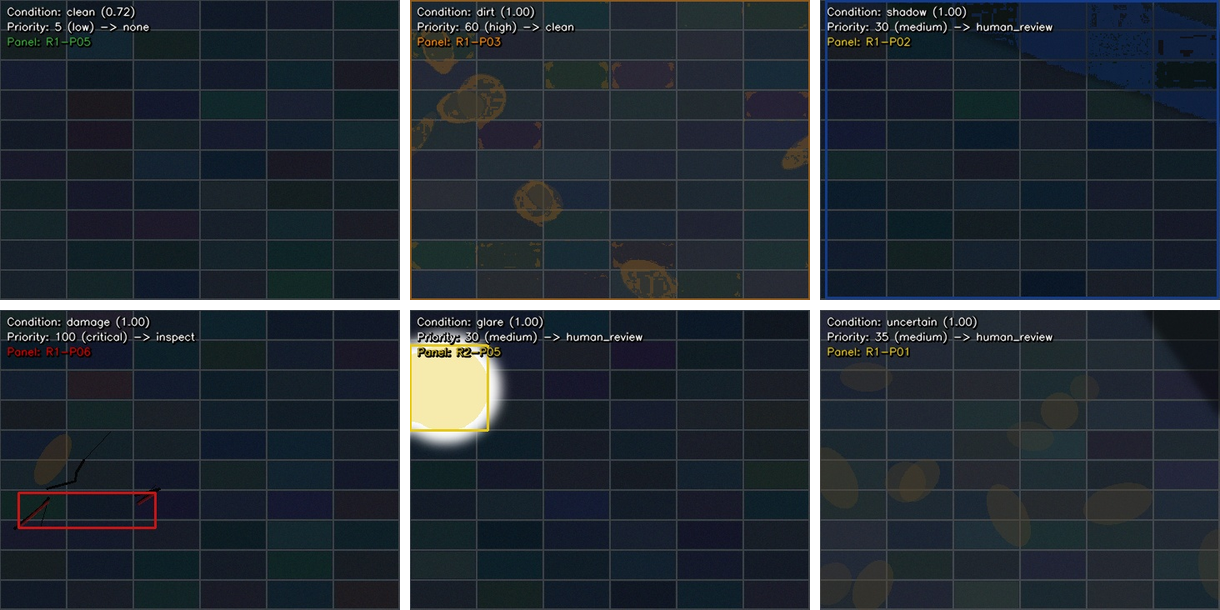
\includegraphics[width=\linewidth]{assets/condition_mosaic.png}
\caption{\footnotesize One annotated synthetic output per required category. Condition, confidence, priority band, and predicted panel are burned into every processed image.}
\label{fig:condition_mosaic}
\end{figure}

On synthetic data, where ground truth exists, this reaches 86.3\% overall: clean and glare both land at 100\%, damage at 88.9\%, and dirt and shadow trail at 75.7\% and 75.0\%, the two conditions closest to each other visually.

I also ran this unmodified classifier against the 119 real photographs. It does not work. Every image comes back uncertain, because real JPEGs carry texture and lighting noise on every frame, which clears every threshold simultaneously and leaves nothing for the tie-break to decide between.

\begin{figure}[!t]
\centering
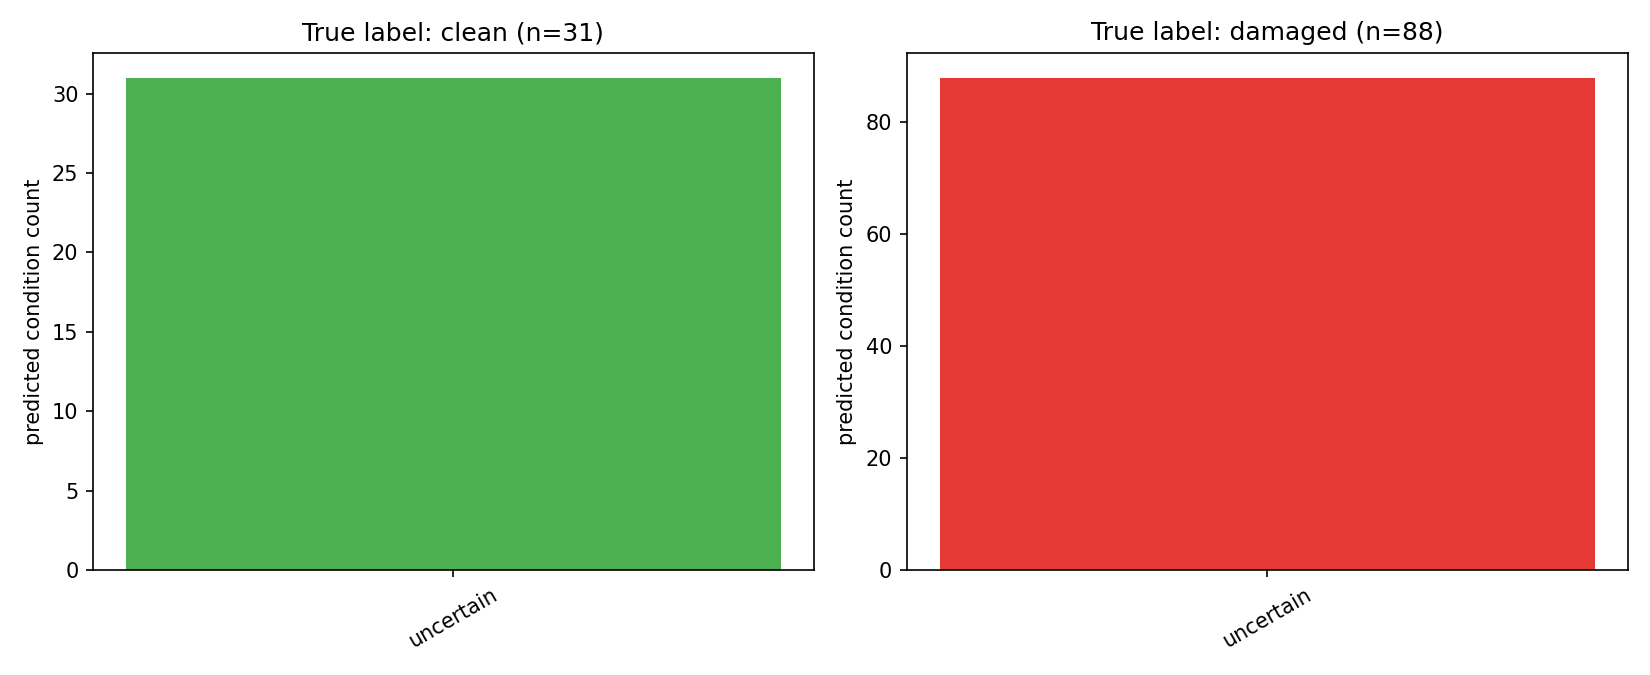
\includegraphics[width=\linewidth]{assets/external_summary.png}
\caption{\footnotesize Zero-shot rule classifier against all 119 real photographs. Every prediction lands on uncertain, for both true-clean and true-damaged images alike.}
\label{fig:external_summary}
\end{figure}

I tried recalibrating thresholds per batch, using each image's own feature percentiles instead of the fixed synthetic values. That made predictions non-degenerate, but the resulting accuracy, 23.9\%, was worse than simply guessing the majority class (73.9\%), so I reverted it rather than count it as progress.

What worked instead was a supervised classifier, logistic regression, five-fold cross-validated, standardized only within each training fold, on the same ten features. It reaches 86.6\% accuracy (Wilson 95\% CI 79.3--91.6\%) telling clean from damaged. Fig.~\ref{fig:external_mosaic} shows three examples: a clean row correctly called clean at 0.99 confidence, a shattered panel correctly called damaged at 0.99, and a genuine miss, a panel covered in dirt and debris that Sunnybotics' own folders label \emph{damaged}, which the model calls clean at 0.53, essentially a coin flip. I read that last case as informative rather than embarrassing: it suggests Sunnybotics' damage label covers soiling as well as breakage, a labeling detail I would not have found without looking at the actual misclassified photo.

\begin{figure}[!t]
\centering
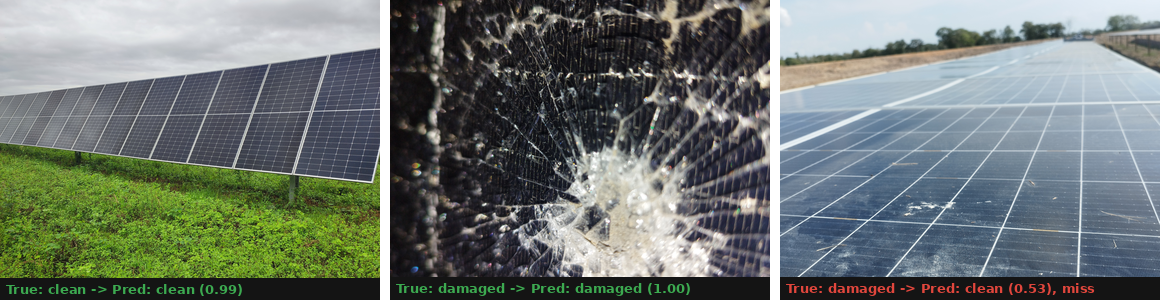
\includegraphics[width=\linewidth]{assets/external_mosaic.png}
\caption{\footnotesize Supervised classifier on real photographs: a confident correct clean call, a confident correct damaged call, and an honest miss on a soiled panel Sunnybotics labels damaged.}
\label{fig:external_mosaic}
\end{figure}

\section{Priority Scoring}
The score branches on the full set of detected issues, not only whichever condition the classifier decided was dominant. A secondary damage signal, even a weak one, should not get buried under a more confident dirt or shadow reading, since missing a real crack is a worse mistake than an extra false alarm.

\begin{table}[!t]
\centering
\caption{\footnotesize Priority score by trigger.}
\label{tab:priority}
\begin{tabularx}{\linewidth}{@{}lXc@{}}
\toprule
\textbf{Trigger} & \textbf{Score rule} & \textbf{Action}\\
\midrule
Unusable image & flat 70 & recapture\\
Damage (any conf.) & $70+30\cdot\text{conf}_{\text{dmg}}$ & inspect\\
Uncertain & flat 35 & human\_review\\
Dirt (dominant) & $20+55\cdot\overline{\text{area}}$ & clean\\
Shadow / glare & flat 30 & human\_review\\
Clean & flat 5 & none\\
\bottomrule
\end{tabularx}
\end{table}

Dirt scores in proportion to the measured area of soiling rather than classifier confidence: a small confident patch and a large uncertain one call for different responses. Damage floors high regardless of what else is in the frame, since a missed structural problem costs more than an unnecessary inspection. The score is independent of how confident the panel association was; a high-priority finding on an ambiguous panel ID gets flagged in the reason text rather than folded into the score itself.

\section{Assumptions}
A few things are worth stating plainly. Synthetic coordinates come from a farm layout projected into local east-north-up coordinates, with GPS jitter, bias, and odometry noise added on top, documented in \texttt{farm\_layout.py} and \texttt{simulate\_mission.py} rather than presented as real telemetry. The external dataset carries none of this metadata; ingestion, association, and export all check which columns are actually present before deciding what is required. Detection thresholds are calibrated once, on synthetic renders, and used unchanged in both modes, a deliberate transfer test, and Section VI is what happens when it is asked to do more than it can.

\section{Failure Cases and Limitations}
Two separate mechanisms inject broken images into the synthetic set, and they do not share a count. Five cases are injected deterministically every run: a missing file, a truncated JPEG, a GPS dropout, an out-of-range coordinate, and a capture missing its mission ID. Separately, about 3\% of captures (3 images currently) get a random visual corruption: heavy blur, blackout, or overexposure. That is eight distinct broken images, not one set of five. Only five are actually rejected before condition analysis runs, the missing file, the truncated one, and the three corrupted-visual cases; the other three stay readable and instead exercise the association layer's odometry fallback. None of the eight crash the pipeline.

Beyond the injected cases, 51 of 100 synthetic associations come back ambiguous rather than matched, by design. The real-photo zero-shot failure from Section III is the more important result of the two: it is the kind of failure a system tested only against its own simulated data would never surface.

\section{Planned Improvements}
The Kalman filter currently detects GPS bias but does not correct it; adding a bias term to the state would let it estimate and remove that error instead of only widening its uncertainty around it. ``Panel not visible'' is approximated today by the same blackout and blur checks used elsewhere, and a dedicated occlusion detector would fit better. The supervised classifier distinguishes only clean from damaged, since that is the only label Sunnybotics' folders provide; extending it to the full five-category schema would need labeled real examples of dirt, shadow, and glare that do not yet exist.

\section{Answers to the Required Questions}

\textit{How do you guarantee that each photo is linked to the correct panel, given 1--3\,m of GPS error?} I do not guarantee it in the strict sense; I try to make the system honest about when it cannot be sure. Section II covers the mechanism: Kalman-fused GPS and odometry, a softmax posterior over known panel positions, and four checks that downgrade to ambiguous rather than commit. What matters most is the result: on the synthetic set, the top-1 guess was correct 100\% of the time, in both the matched and ambiguous groups.

\textit{How do you detect that an image is unusable?} Three cheap checks run before condition analysis: a forced full decode with PIL's \texttt{.load()} rather than \texttt{.verify()}, which I found empirically does not catch a truncated file; a pixel standard-deviation check for blackout or overexposure; and a Laplacian-variance check for blur. There is no dedicated ``panel not visible'' detector yet, a real gap noted in Section VII.

\textit{How would you tell real dirt apart from a temporary shadow?} Dirt and shadow are measured as two separate features from the start. Where the same panel is captured across two missions with a confident association in both, that repetition helps: a signal present in only one mission is more likely a shadow, one present in both is more likely persistent dirt, though this only adjusts confidence and never overrides the single-image classification. Real photographs lack that multi-mission structure, so there the same two measurements instead feed the supervised classifier's learned weighting.

\textit{What metrics would you use without complete ground truth?} Report a range rather than a single number: the Wilson interval on the real classifier, 86.6\% [79.3, 91.6], matters more than the point estimate at this sample size. Track the abstention rate (ambiguous or uncertain, 51\% plus 14\% in synthetic mode) as a metric in its own right, since a well-calibrated system should decline exactly where it is genuinely unsure. And check whether confidence means anything by stratifying accuracy by it: on real data, the top 20\% most confident predictions were 95.8\% accurate against 75.0\% for the bottom 20\%.

\textit{Which parts would run on the robot versus in the cloud?} Capture, GPS/odometry fusion, panel association, and unusable-image screening belong on the robot: low latency, no dependence on connectivity, and a bad frame gets retaken immediately rather than discovered hours later. Feature extraction, classification, the cross-mission temporal check, and the export/dashboard layer fit the cloud better, benefiting from centralized retraining as labeled data accumulates.

\textit{What is the biggest technical risk, and how would this scale to thousands of panels?} The biggest risk is exactly what Section III shows: thresholds calibrated on one image distribution do not transfer to real optical conditions. At scale that becomes a large backlog of uncertain results rather than confidently wrong ones, a safer failure mode but still not a free one. The path I would take is the supervised classifier validated here: per-image inference parallelizes trivially across a farm, and the Kalman association runs in constant time per capture, so cost scales with feature-extraction compute and storage, not algorithmic complexity.

\section{Validation and Additional Work}
Forty automated tests cover the pipeline, the external-dataset adapter, and the supervised classifier, and both modes reproduce byte-identical output on rerun. The cross-validation tests guarding against label leakage were mutation-tested: I reintroduced two leaks (held-out labels passed into scoring; fitting on the full dataset instead of the training fold) one at a time, confirmed each was caught, then reverted both, the difference between a test that looks right and one I have watched fail.

Beyond the required features, this includes a simulated GPS and odometry route across two full missions, automatic detection of unusable images, and a recommended-action layer (clean, inspect, human review, recapture, none) tied to the priority formula.

\begin{figure}[H]
\centering
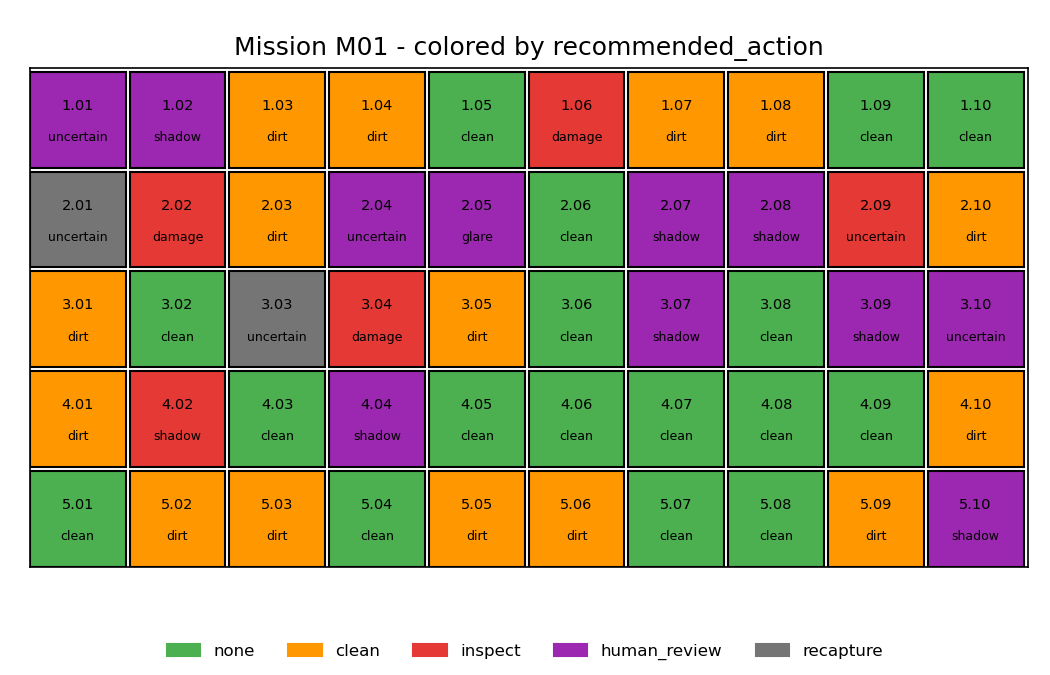
\includegraphics[width=0.62\linewidth]{assets/farm_grid_m01.png}
\caption{\footnotesize Farm-grid dashboard, mission 1: panel ID, condition, and recommended action per cell, giving full traceability from image to location to diagnosis. It also ships as a filterable interactive HTML page.}
\label{fig:farm_grid}
\end{figure}

\end{document}
